% presentation
%\documentclass[compress,draft]{beamer}
\documentclass[compress,aspectratio=1610]{beamer}
% handout
%\documentclass[handout]{beamer}

\usepackage{../mtex,fancyvrb,booktabs,tasks}
\usepackage{tikz,pgfplots}
\usepackage{tikz-3dplot}
\usetikzlibrary{angles,quotes}
%\usepackage{subfigure}
\usepackage[labelformat=empty]{subcaption}
\captionsetup{compatibility=false}
%\usepackage[inline]{enumitem}
% \newcommand\paraitem{%
%   \;
%   \makebox[\labelwidth][r]{%
%     \makelabel{%
%       \usebeamertemplate{itemize \beameritemnestingprefix item}}}\hskip\labelsep}



\author{R. Hielscher}

\title{Matlab Basics and General Concepts of the MTEX Toolbox}

\institute{Faculty of Mathematics and Computer Science,\\
	TU Bergakademie Freiberg, Germany}

\date{2024}


\renewcommand<>{\ul}[1]{
  \alt#2{\underline{#1}}{#1}
}

\begin{document}

\newcommand{\labelitemi}{%
  \begingroup%
  \leavevmode%
  \protect\usebeamerfont*{itemize item}%
  \protect\usebeamercolor[fg]{itemize item}%
  \protect\usebeamertemplate**{itemize item}%
  \endgroup%
 }

 \settasks{
   item-indent = 2em ,
   label-width = 1em ,
   label-offset = 0pt
}

\begin{frame}
  \maketitle{}


  % Mathematician -> what is the audiance?
  % why do I teach texture analysis ?
  % lectures -> Theory
  % exercises -> compute things yourself using MTEX
  % --> Pool
  % examination -> oral
  % after lecture: MTEX workshop

\end{frame}

\begin{frame}
  \frametitle{MTEX - A tool for calculating with orientation dependent properties}

  \calculatespace%
  
  \begin{columns}[c,onlytextwidth]
    \begin{column}{0.4\textwidth}

      \begin{itemize}
        \item<1-> crystal geometry
        \item<2-> EBSD data
        \item<3-> grains, grain boundaries
        \item<4-> XRD data
        \item<5-> orientation distribution function
        \item<6-> texture simulations
        \item<10-> tensorial properties
        \item<11-> elastic / plastic deformation
        \item<12-> misorientations / twinning
        \item<13-> phase transformations
        \item<14-> parent grain reconstruction
        \end{itemize}

        \medskip
        
        \uncover<15>{\structure{Focus: basics, generality, speed}}
        
    \end{column}
    \begin{column}{0.5\textwidth}
      \begin{center}
        \only<1>{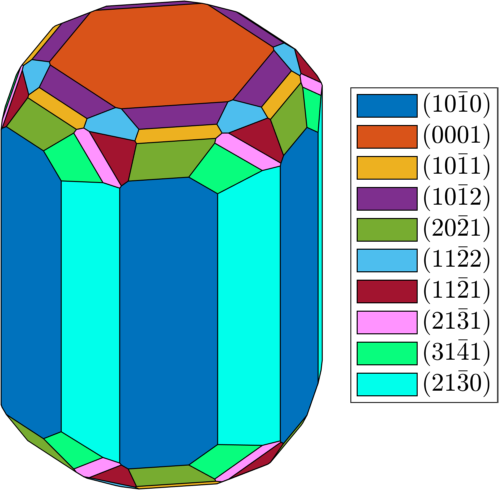
\includegraphics[width=0.9\textwidth]{pic/apatite}}
        \only<2>{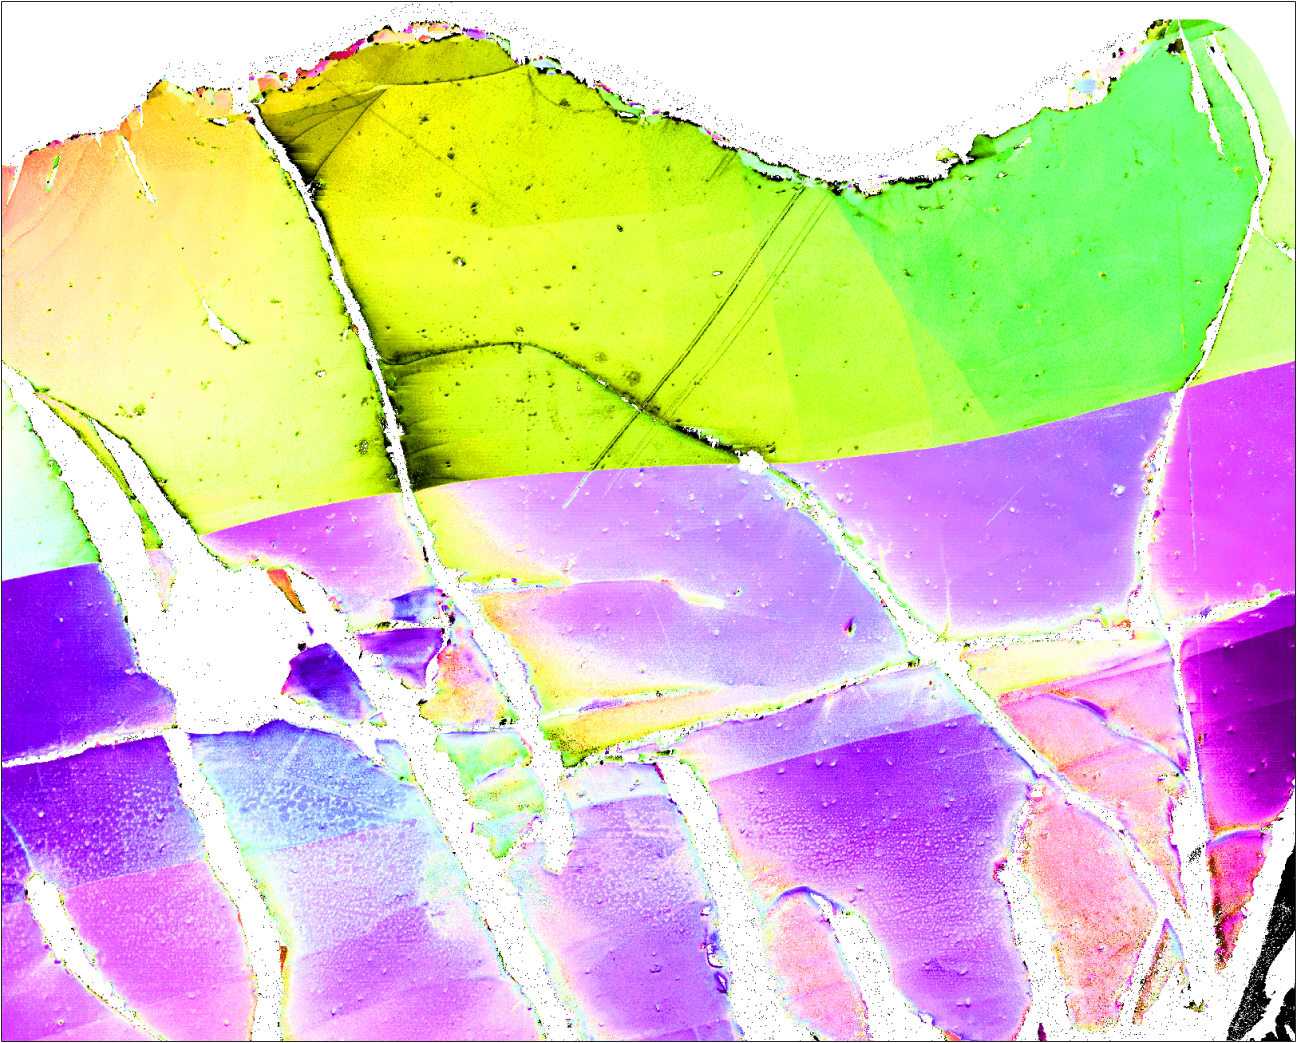
\includegraphics[angle=90,width=0.8\textwidth]{pic/forsterite}}
        % \only<3>{\centering
        % \includegraphics[width=0.7\textwidth]{pic/532EBSD}}
        \only<3>{\centering
          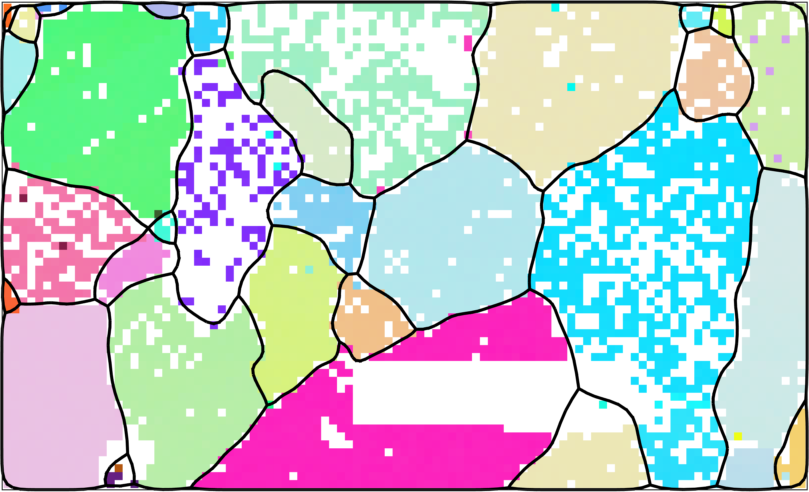
\includegraphics[angle=90,width=0.6\textwidth]{pic/ebsdGrain2}}
        \only<4>{\centering
          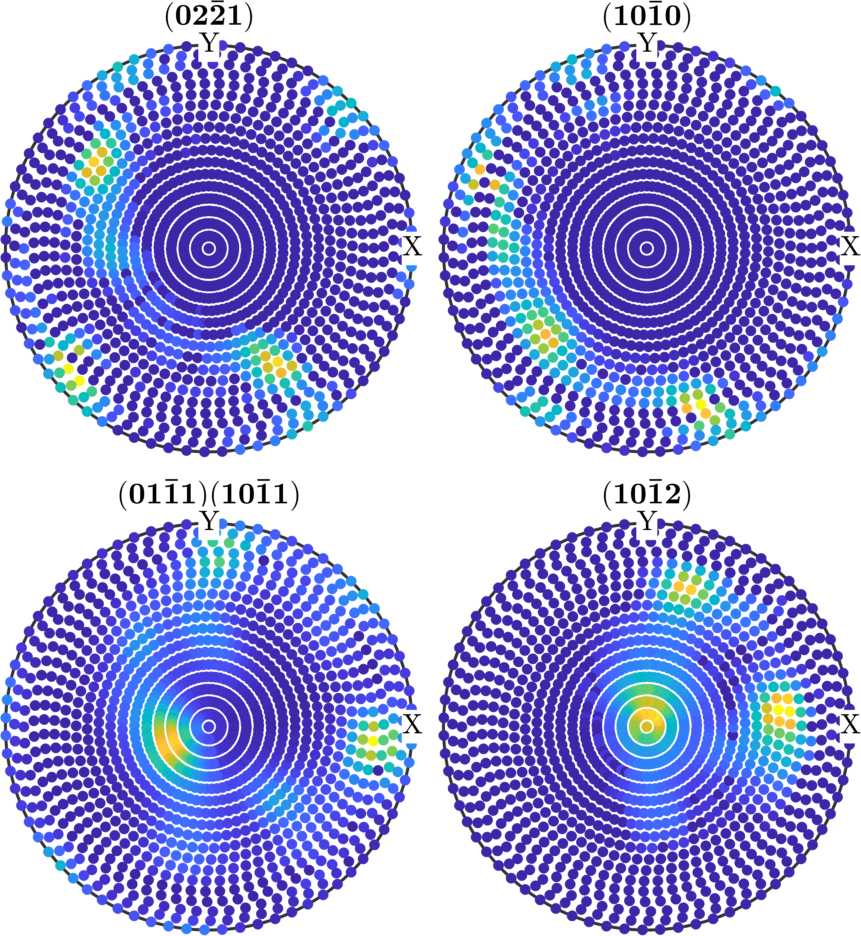
\includegraphics[width=0.9\textwidth]{pic/pfDubna}}
        \only<5>{\centering
          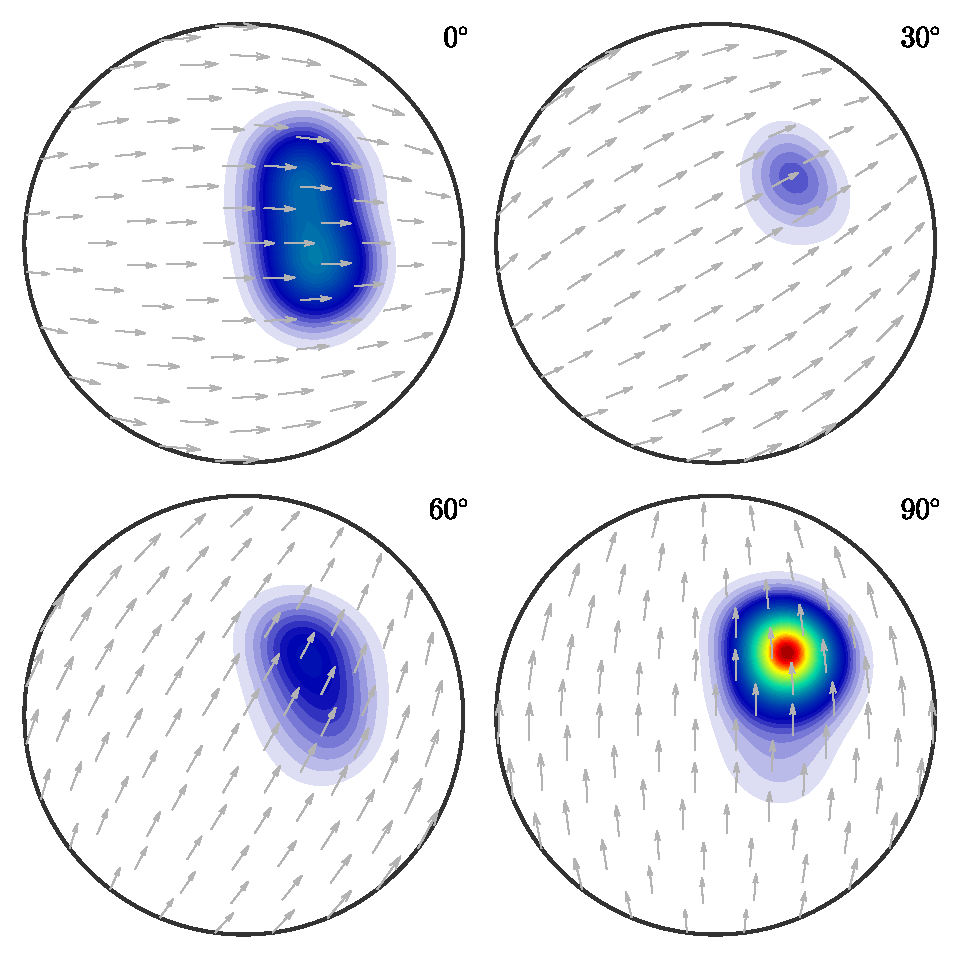
\includegraphics[width=0.95\textwidth]{pic/odfDubna.pdf}}
        \only<6>{\centering
          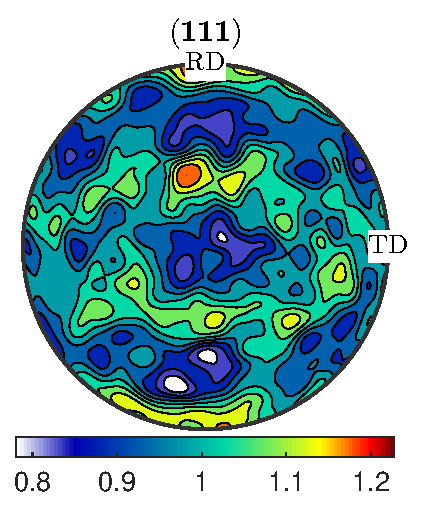
\includegraphics[width=0.7\textwidth]{pic/rolling/rolling111_1.pdf}}
        \only<7>{\centering
          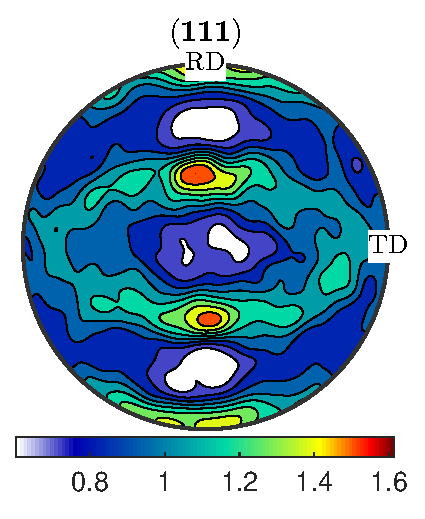
\includegraphics[width=0.7\textwidth]{pic/rolling/rolling111_3.pdf}}
        \only<8>{\centering
          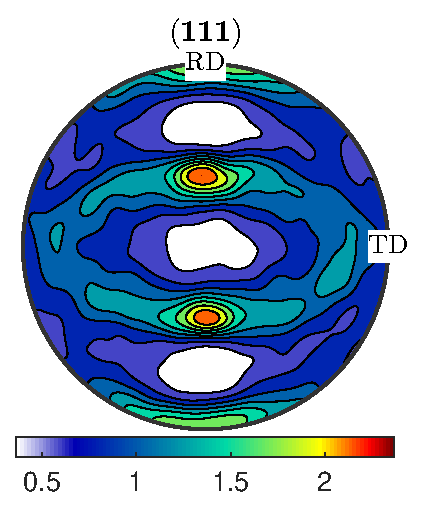
\includegraphics[width=0.7\textwidth]{pic/rolling/rolling111_6.pdf}}
        \only<9>{\centering
          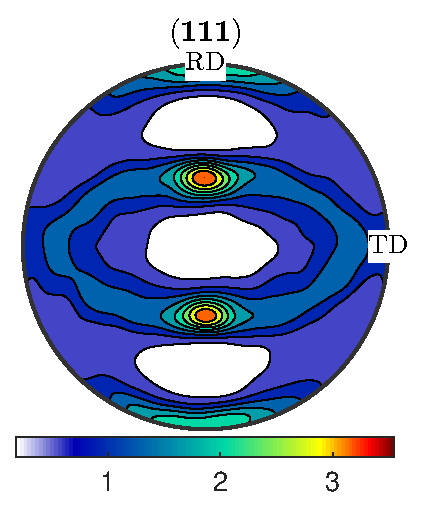
\includegraphics[width=0.7\textwidth]{pic/rolling/rolling111_10.pdf}}
        \only<10>{\centering
          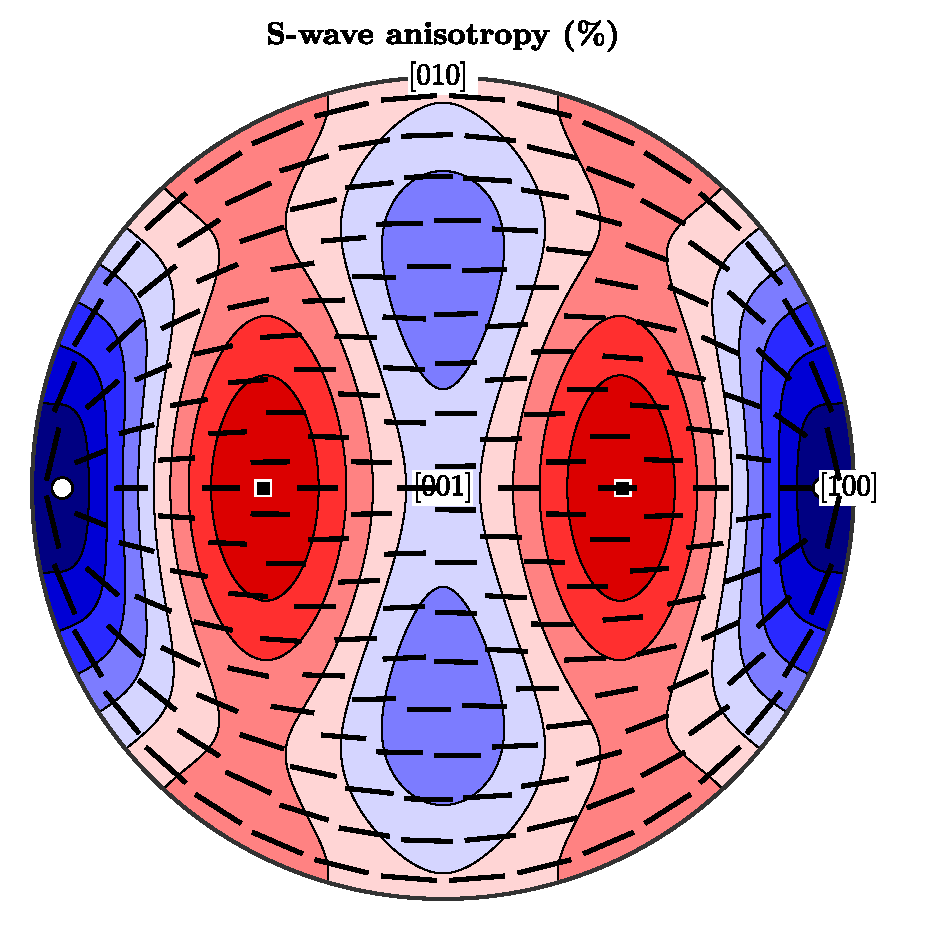
\includegraphics[width=0.85\textwidth]{pic/velocity.pdf}}
        \only<11>{\centering
          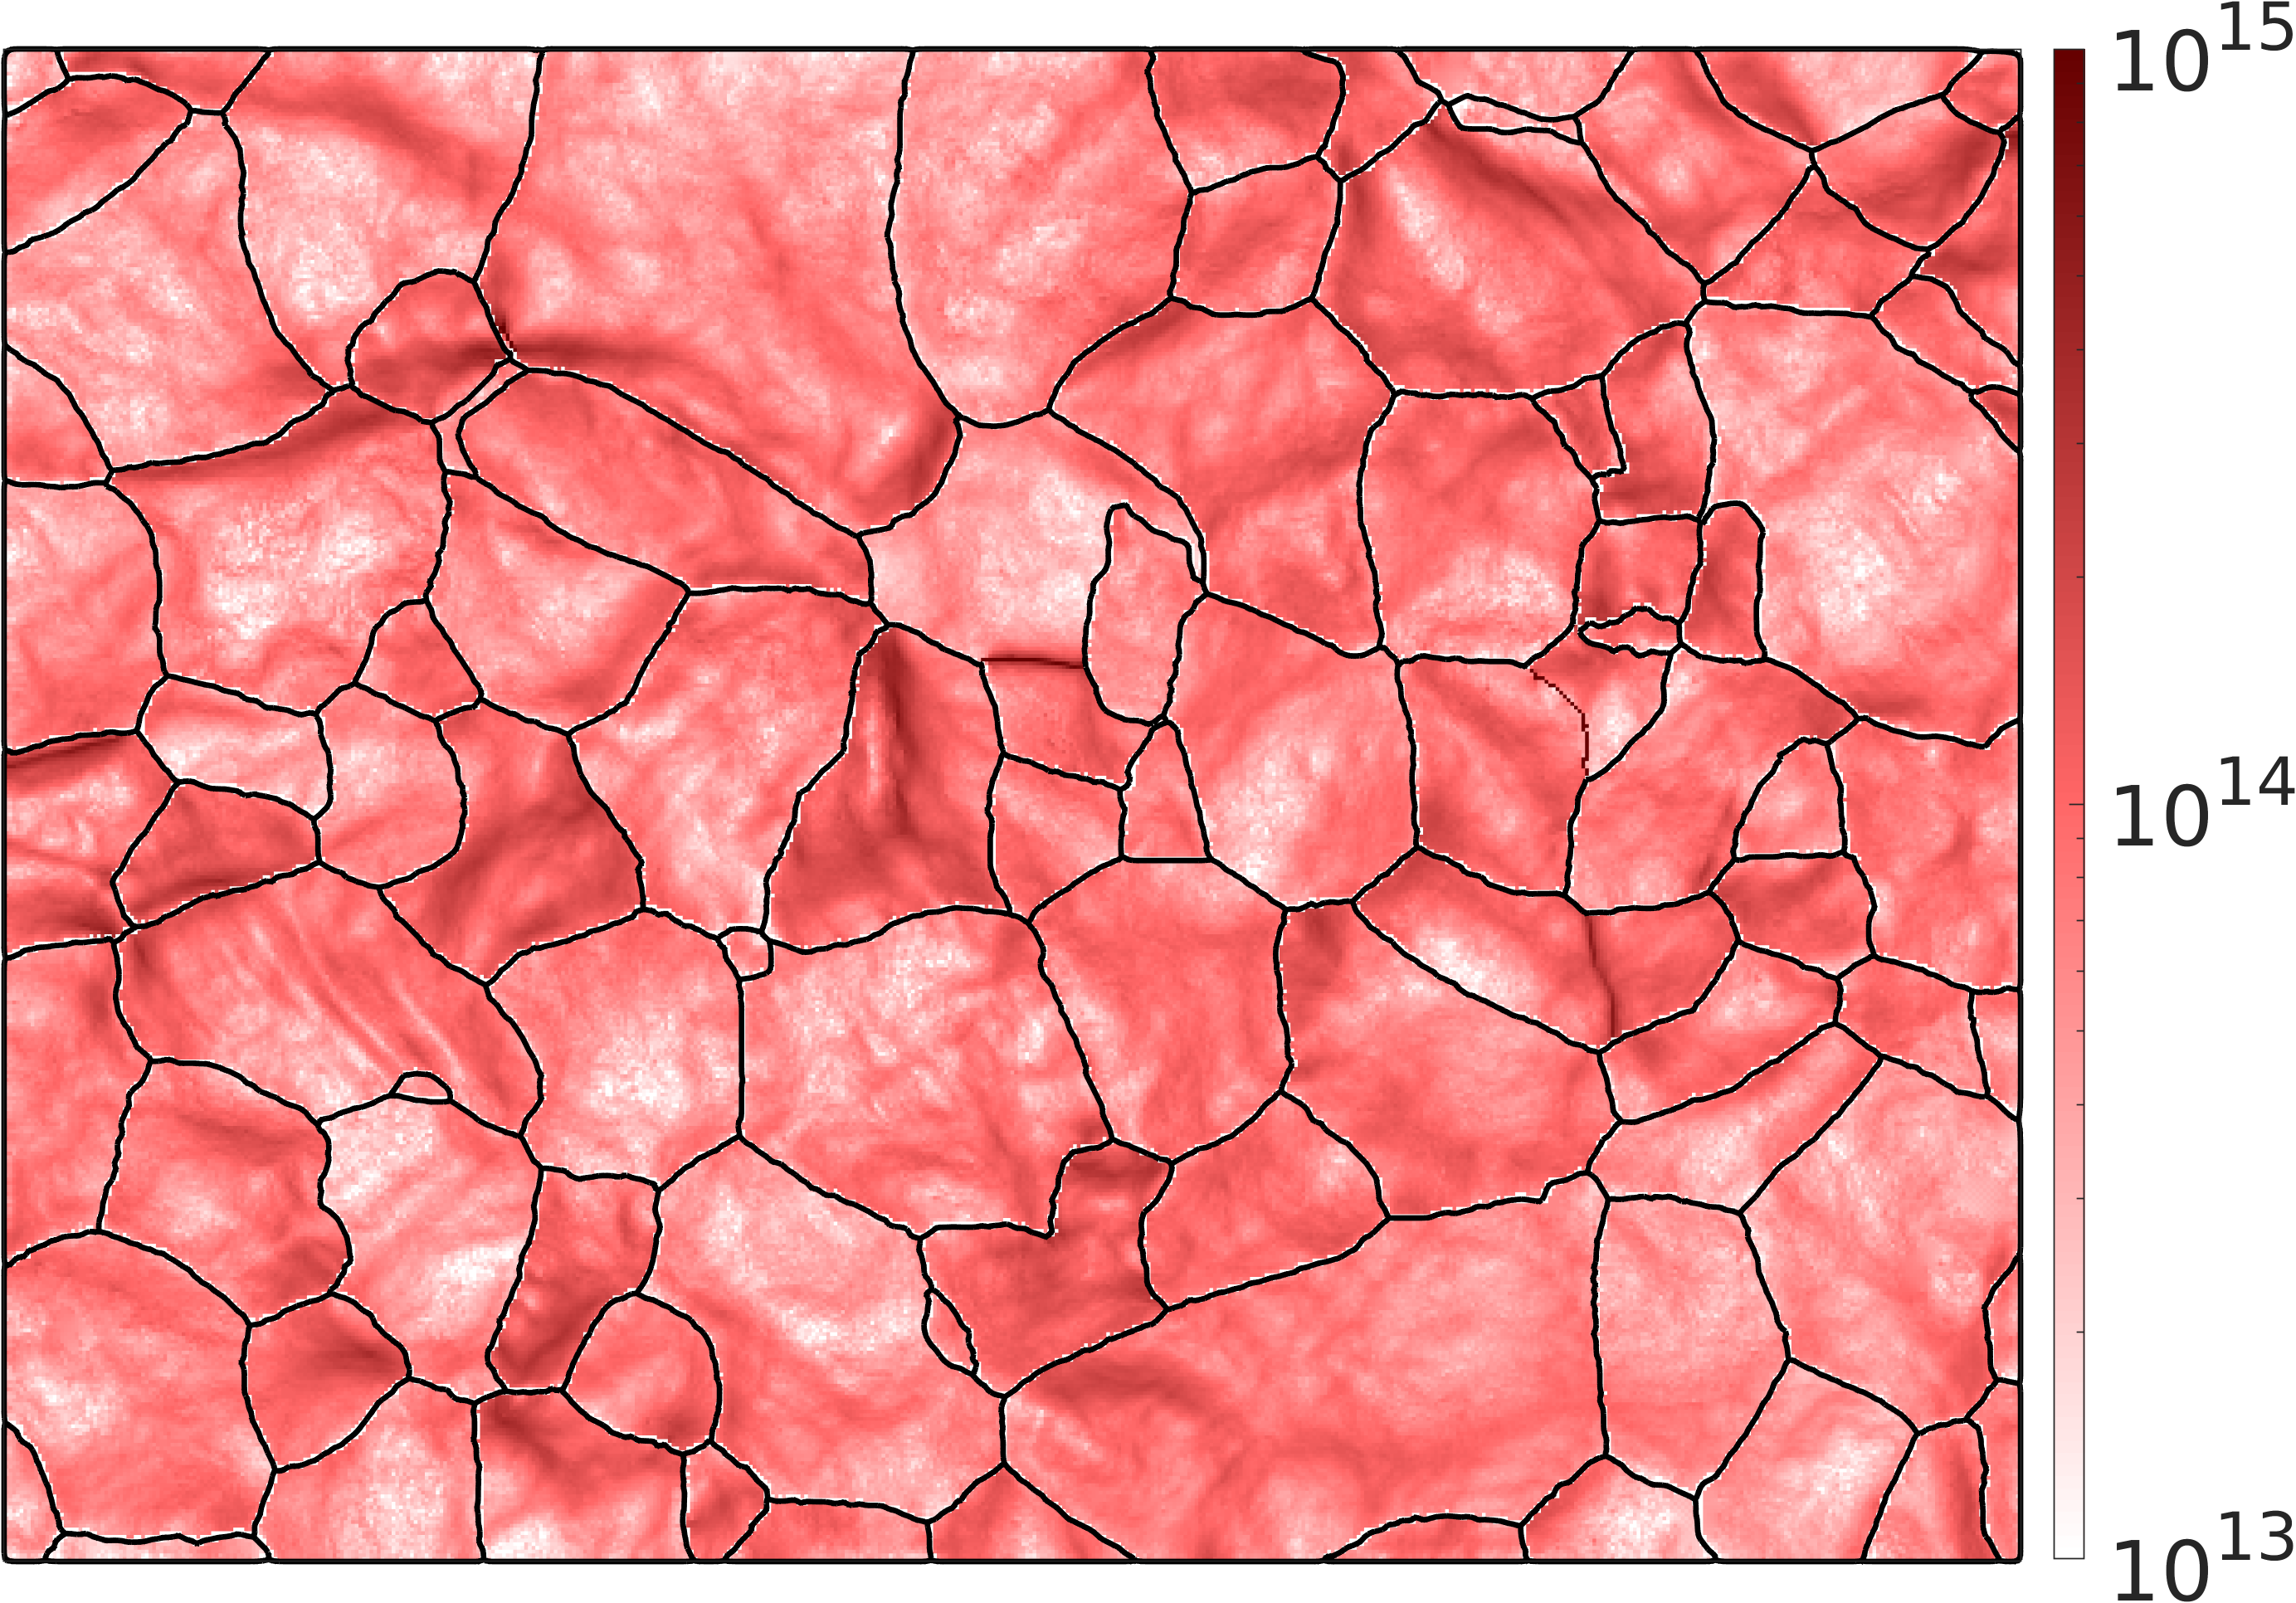
\includegraphics[width=\textwidth]{pic/ebsdSGND}}
      \end{center}
    \end{column}
  \end{columns}
\end{frame}

\begin{frame}
  \frametitle{MTEX an Open Source Toolbox}

  \begin{block}{Large, well documented, tested}
    \begin{tasks}[style=itemize](2)
     \task 13 years of development
     \task 1000 functions
     \task 40 000 lines of code, 33 percent comments
     \task 14 reference paper, about 2000 references
     \task 2000 downloads per version
     \task 1000 help pages
     \task* add-ons: MTEX GUI, MTEX2Gmsh, Stabix,
     CrystalAligner, phaseSegmenter
    \end{tasks}
  \end{block}

  \begin{block}{A Teaching Tool}
      \begin{tasks}[style=itemize](2)
     \task everything can be visualized
     \task everything can be manipulated
     \task* everything can be combined with everything
%     \task no black box solutions
   \end{tasks}
 \end{block}

 \begin{block}{Free and open software}
   \begin{tasks}[style=itemize](3)
     \task free to use
     \task free to modify
     \task very nice comunity
   \end{tasks}
 \end{block}
\end{frame}



\begin{frame}[fragile]
  \frametitle{MTEX - A Matlab based scripting language}


  \begin{columns}
    \begin{column}{0.62\textwidth}
      %\structure{An example:}
\begin{lstlisting}[style=input]
% load data
ebsd = EBSD.load('Emsland_plessite.ctf')

% plot data
plot(ebsd('Fe'),ebsd('Fe').orientations)

% reconstruct grains
th = 5*degree;
grains = calcGrains(ebsd,'threshold',th)

% find largest grain
[m,id] = max(grains.area)

% plot largest grain
plot(grains(id).boundary,'linewidth',2)
\end{lstlisting}
      \end{column}
      \begin{column}{0.35\textwidth}
        \begin{overlayarea}{\textwidth}{8cm}

          \begin{onlyenv}<2> \structure{Why scripts?}
            \begin{itemize}
            \item reproducible results
            \item easy to document
            \item templates for common tasks
            \item extensively customizable
            \item batch processing of many data sets
            \item repeated calculations with different parameters
            \end{itemize}
          \end{onlyenv}


          \begin{onlyenv}<2> \structure{Best practice}
            \begin{itemize}
            \item comment your scripts
            \item short scripts
            \item function for repeated tasks
            \item avoid loops
            \end{itemize}
          \end{onlyenv}


      \end{overlayarea}
    \end{column}

    \end{columns}
\end{frame}




\begin{frame}
  \frametitle{MTEX Resources}

  \begin{columns}
    \begin{column}{0.3\textwidth}
      \begin{tasks}[style=itemize]
        \task documentation \task function reference \task examples \task user
        scripts \task discussion forum
      \end{tasks}
    \end{column}
    \begin{column}{0.7\textwidth}

    \end{column}
  \end{columns}
\end{frame}

\begin{frame}
  \frametitle{Matlab}

  show this live:

  \begin{itemize}
  \item matrices
  \item command line
  \item workspace
  \end{itemize}

\end{frame}

\begin{frame}[fragile]
  \frametitle{Three dimensional vectors}

  \begin{overlayarea}{\textwidth}{\textheight}
    Three dimensional vectors are given by there coordinates with respect to a
    orthogonal coordinate system $\vec X, \vec Y, \vec Z$
  \begin{equation*}
    \vec r = x \cdot \vec X + y \cdot \vec Y + z \cdot \vec Z
  \end{equation*}

  \pause

  For general vectors, MTEX does \textbf{not} care about the coordinate
  system, but works only with the coordinates.

  \begin{columns}
    \begin{column}{0.6\textwidth}
      \begin{lstlisting}[style=input]
r = vector3d(1,2,3)
  \end{lstlisting}
      \begin{onlyenv}<2|handout:0>
        \vspace{-0.3cm}
\begin{lstlisting}[style=output]
r = /+vector3d+/ (show methods, plot)
  size: 1 x 1
  x y z
  1 2 3
\end{lstlisting}
      \end{onlyenv}

      \medskip

      \begin{onlyenv}<3-> The alignment of the coordinate system is only
        important when plotting data
      \end{onlyenv}
      \begin{onlyenv}<3|handout>
\begin{lstlisting}[style=input]
plotx2north, plotzOutOfPlane
plot(r)
\end{lstlisting}
      \end{onlyenv}
      \begin{onlyenv}<4>
\begin{lstlisting}[style=input]
plotx2east, plotzOutOfPlane
plot(r)
\end{lstlisting}
      \end{onlyenv}
    \end{column}
    \begin{column}{0.37\textwidth}
      \only<3>{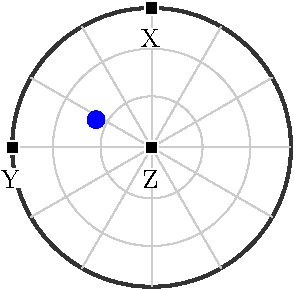
\includegraphics[width=3.5cm]{pic/vectorNorth}}%
      \only<4|handout:0>{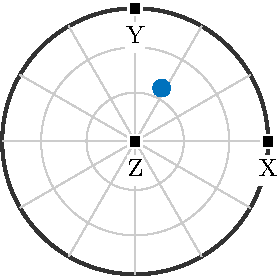
\includegraphics[width=3.5cm]{pic/vectorEast}}
    \end{column}
  \end{columns}

%  \pause
  \medskip

  \begin{onlyenv}<4> Only for directions relative to the crystal coordinate
    system the reference frame is considered.
  \end{onlyenv}


\end{overlayarea}
\end{frame}

\begin{frame}[fragile,fragile,fragile]
  \frametitle{Defining vectors}

  \begin{overlayarea}{\textwidth}{0.95\textwidth}
    \vspace{-0.1cm}
    \begin{columns}
      \begin{column}{0.6\textwidth}
        predefined vectors \vspace{-0.15cm}
\begin{lstlisting}[style=input]
vector3d.X, vector3d.Y, vector3d.Z
\end{lstlisting}

        \pause \medskip

        polar coordinates
        $\vec r = (\sin \theta \cos \rho,\sin \theta \sin \rho,\cos
        \theta)^{t}$ \vspace{-0.15cm}
\begin{lstlisting}[style=input]
theta = 90 * degree; rho = 45 * degree;
r = vector3d.byPolar(theta,rho)
\end{lstlisting}

        \alert{In MTEX all angles are in radiant!}

      \end{column}
      \begin{column}{0.37\textwidth}
        \vspace{-1cm}
%Angle Definitions
%-----------------

%set the plot display orientation
%syntax: \tdplotsetdisplay{\theta_d}{\phi_d}
\tdplotsetmaincoords{60}{25}

%define polar coordinates for some vector
%TODO: look into using 3d spherical coordinate system
\pgfmathsetmacro{\rvec}{1}
\pgfmathsetmacro{\thetavec}{60}
\pgfmathsetmacro{\phivec}{30}

%start tikz picture, and use the tdplot_main_coords style to implement the display
\begin{tikzpicture}[scale=1.75,tdplot_main_coords]

%set up some coordinates
%-----------------------
\coordinate (O) at (0,0,0);
\fill (O) circle[radius=1pt] node[below left] {O};

%determine a coordinate (P) using (r,\theta,\phi) coordinates.
%syntax: \tdplotsetcoord{Coordinate name without parentheses}{r}{\theta}{\phi}
\tdplotsetcoord{P}{\rvec}{\thetavec}{\phivec}
\fill (P) circle[radius=1pt] node[anchor=south west] {P};

%draw figure contents
%--------------------

%draw the main coordinate system axes
\draw[thick,->] (0,0,0) -- (0,1.2,0) node[anchor=south]{$y$};

%draw the angle \phi, and label it
%syntax: \tdplotdrawarc[coordinate frame, draw options]{center point}{r}{angle start}{angle end}{label options}{label}
%\tdplotdrawarc[fill=green!20]{(O)}{0.7}{0}{\phivec}{anchor=north}{$\rho$}

\draw [fill=blue!20, domain=0:30] (0,0) -- plot (0.7*cos \x, 0.7*sin \x) -- cycle;
\draw[blue!50!black] (0.6,0.1) node{$\rho$};

\tdplotsetthetaplanecoords{\phivec}
\draw[tdplot_rotated_coords] [fill=green!20, domain=0:60]
    (0,0) -- plot (0.6*cos \x, 0.6*sin \x) -- cycle;
\draw[green!50!black] (-0.1,0.5) node{$\theta$};

% set the rotated coord system so the x'y' plane coincides with the"theta plane" of the main coord system
%syntax: \tdplotsetthetaplanecoords{\phi}
%\tdplotsetthetaplanecoords{\phivec}

%draw theta arc and label, using rotated coordinate system
%\tdplotdrawarc[tdplot_rotated_coords]{(0,0,0)}{0.2}{0}{\thetavec}{anchor=south
%  west}{$\theta$}

%draw some dashed arcs, demonstrating direct arc drawing
\draw[dashed,tdplot_rotated_coords] (\rvec,0,0) arc (0:360:\rvec);
\draw[dashed,blue!50!black] (\rvec,0,0) arc (0:360:\rvec);

%draw a vector from origin to point (P), projection on xy plane, and a connecting line
\draw[-stealth,very thick] (O) -- (P);
\draw[thick] (O) -- (Pxy);
\draw[thick] (P) -- (Pxy);


\draw[thick,->] (0,0,0) -- (1.2,0,0) node[anchor=west]{$x$};
\draw[thick,->] (0,0,0) -- (0,0,1.1) node[anchor=south]{$z$};


\end{tikzpicture}

      \end{column}
    \end{columns}
  \pause \medskip

  combine vectors
  \vspace{-0.15cm}
\begin{lstlisting}[style=input]
r = [vector3d.X, vector3d.Y, vector3d(1,1,1)]
\end{lstlisting}

\begin{onlyenv}<3|handout:0>
  \vspace{-.3cm}
\begin{lstlisting}[style=output]
r = /+vector3d+/ (show methods, plot)
  size: 1 x 3
  x y z
  1 0 0
  0 1 0
  1 1 1
\end{lstlisting}
\end{onlyenv}
  \pause \medskip

  importing vectors
  \vspace{-0.15cm}
\begin{lstlisting}[style=input]
r = vector3d.load('file','ColumnNames',{'x','y','z'})
\end{lstlisting}
\begin{onlyenv}<4|handout:0>
  \vspace{-.3cm}
\begin{lstlisting}[style=output]
r = /+vector3d+/ (show methods, plot)
  size: 200 x 1
\end{lstlisting}
\end{onlyenv}

\pause \medskip
random vectors
  \vspace{-0.15cm}
\begin{lstlisting}[style=input]
r = vector3d.rand(100)
\end{lstlisting}

\end{overlayarea}
\end{frame}

\begin{frame}[fragile,fragile]
  \frametitle{Vector Calculations}

  simple algebra
    \vspace{-0.15cm}
\begin{lstlisting}[style=input]
r = 2*vector3d.X - vector3d.Y;
\end{lstlisting}

  \pause \medskip


  basic operations
    \vspace{-0.15cm}
\begin{lstlisting}[style=input]
dot(v1,v2)   % dot product
cross(v1,v2) % cross product
angle(v1,v2) % angle between two vectors
normalize(v) % scale to norm 1
orth(v)      % arbitrary orthogonal vector
\end{lstlisting}

%   \pause \medskip

%   density estimation
%     \vspace{-0.15cm}
% \begin{lstlisting}[style=input]
% sF = calcDensity(v,'halfwidth',5*degree)
% \end{lstlisting}
%     \begin{onlyenv}<3> \vspace{-0.3cm}
% \begin{lstlisting}[style=output]
% sF = /+S2FunHarmonic+/ (show methods, plot)
%  bandwidth: 25
% \end{lstlisting}
%     \end{onlyenv}

  \pause \medskip

  extract properties
    \vspace{-0.15cm}
\begin{lstlisting}[style=input]
r.theta      % polar angle in radiant
r.rho        % azimuth angle in radiant
r.x, r.y, r.z
\end{lstlisting}

\end{frame}


\begin{frame}[fragile]
  \frametitle{Indexing of Vectors}

  \medskip

  \begin{overlayarea}{\textwidth}{0.85\textheight}

    consider a list of vectors
      \vspace{-0.15cm}
    \begin{lstlisting}[style=input]
r = vector3d([0 0 1 1],[1 0 1 1],[1 1 1 0]);
    \end{lstlisting}

    \begin{onlyenv}<1|handout:0>
      \vspace{-.3cm}
      \begin{lstlisting}[style=output]
r = /+vector3d+/ (show methods, plot)
  size: 1 x 4
  x y z
  0 1 1
  0 0 1
  1 1 1
  1 1 0
      \end{lstlisting}
    \end{onlyenv}

    \pause \medskip

    single out the second vector
      \vspace{-0.15cm}
    \begin{lstlisting}[style=input]
r(2)
    \end{lstlisting}

    \begin{onlyenv}<2|handout:0>
      \vspace{-0.3cm}
      \begin{lstlisting}[style=output]
r = /+vector3d+/ (show methods, plot)
  size: 1 x 1
  x y z
  0 0 1
      \end{lstlisting}
    \end{onlyenv}

    \pause \medskip

    single out the second and the fourth vector
      \vspace{-0.15cm}
    \begin{lstlisting}[style=input]
r([2 4])
    \end{lstlisting}
    \begin{onlyenv}<3|handout:0>
      \vspace{-0.3cm}
      \begin{lstlisting}[style=output]
r = /+vector3d+/ (show methods, plot)
  size: 1 x 2
  x y z
  0 0 1
  1 1 0
      \end{lstlisting}
    \end{onlyenv}

  \pause \medskip

  single out vectors by a logical condition
    \vspace{-0.15cm}
    \begin{lstlisting}[style=input]
r(r.x>0)
    \end{lstlisting}
        \begin{onlyenv}<4|handout:0>
          \vspace{-0.3cm}
      \begin{lstlisting}[style=output]
r = /+vector3d+/ (show methods, plot)
  size: 1 x 2
  x y z
  1 1 1
  1 1 0
     \end{lstlisting}
    \end{onlyenv}

    \pause \medskip

    \alert{The above techniques applies also to lists of rotations,
      orientations, tensors, EBSD data, grains, boundary segments, triple
      points, etc.}
  \end{overlayarea}
\end{frame}


\begin{frame}[fragile]
  \frametitle{Changing Vectors}

  \medskip

  \begin{overlayarea}{\textwidth}{0.85\textheight}

    consider again the list of vectors
      \vspace{-0.15cm}
    \begin{lstlisting}[style=input]
r = vector3d([0 0 1 1],[1 0 1 1],[1 1 1 0]);
    \end{lstlisting}

    \begin{onlyenv}<1|handout:0>
      \vspace{-0.3cm}
      \begin{lstlisting}[style=output]
r = /+vector3d+/ (show methods, plot)
  size: 1 x 4
  x y z
  0 1 1
  0 0 1
  1 1 1
  1 1 0
      \end{lstlisting}
    \end{onlyenv}

    \pause \medskip

    replace the second vector by another vector
  \vspace{-0.15cm}
\begin{lstlisting}[style=input]
r(2) = vector3d.Y
    \end{lstlisting}

    \begin{onlyenv}<2|handout:0>
      \vspace{-0.3cm}
      \begin{lstlisting}[style=output]
r = /+vector3d+/ (show methods, plot)
  size: 1 x 4
  x y z
  0 1 1
  0 1 0
  1 1 1
  1 1 0
      \end{lstlisting}
    \end{onlyenv}

    \pause \medskip

    remove the second vector completely
      \vspace{-0.15cm}
    \begin{lstlisting}[style=input]
r(2) = []
    \end{lstlisting}
    \begin{onlyenv}<3|handout:0>
      \vspace{-0.3cm}
      \begin{lstlisting}[style=output]
r = /+vector3d+/ (show methods, plot)
  size: 1 x 3
  0 1 1
  1 1 1
  1 1 0
      \end{lstlisting}
    \end{onlyenv}

  \pause \medskip

  change the x coordinate of all vectors
    \vspace{-0.15cm}
    \begin{lstlisting}[style=input]
r.x = 0
    \end{lstlisting}
        \begin{onlyenv}<4|handout:0>
          \vspace{-0.3cm}
      \begin{lstlisting}[style=output]
r = /+vector3d+/ (show methods, plot)
  size: 1 x 3
  0 1 1
  0 1 1
  0 1 0
     \end{lstlisting}
    \end{onlyenv}

    \pause \medskip

    \alert{The above techniques applies also to pole figure data,
    orientations, EBSD data, grains, etc.}
  \end{overlayarea}

\end{frame}

\begin{frame}[label=current]
  \frametitle{Spherical Projections}

  \begin{columns}

\begin{column}{0.45\textwidth}
  \begin{center}
    spherical polar coordinates
    \begin{equation*}
      (x,y,z) = (\cos \rho \sin \theta, \sin \rho \sin \theta, \cos \theta)
    \end{equation*}

%Angle Definitions
%-----------------

%set the plot display orientation
%syntax: \tdplotsetdisplay{\theta_d}{\phi_d}
\tdplotsetmaincoords{60}{25}

%define polar coordinates for some vector
%TODO: look into using 3d spherical coordinate system
\pgfmathsetmacro{\rvec}{1}
\pgfmathsetmacro{\thetavec}{60}
\pgfmathsetmacro{\phivec}{30}

%start tikz picture, and use the tdplot_main_coords style to implement the display
\begin{tikzpicture}[scale=2.8,tdplot_main_coords]

%set up some coordinates
%-----------------------
\coordinate (O) at (0,0,0);
\fill (O) circle[radius=1pt] node[below left] {O};

%determine a coordinate (P) using (r,\theta,\phi) coordinates.
%syntax: \tdplotsetcoord{Coordinate name without parentheses}{r}{\theta}{\phi}
\tdplotsetcoord{P}{\rvec}{\thetavec}{\phivec}
\fill (P) circle[radius=1pt] node[anchor=south west] {P};

%draw figure contents
%--------------------

%draw the main coordinate system axes
\draw[thick,->] (0,0,0) -- (0,1.2,0) node[anchor=south]{$y$};

%draw the angle \phi, and label it
%syntax: \tdplotdrawarc[coordinate frame, draw options]{center point}{r}{angle start}{angle end}{label options}{label}
%\tdplotdrawarc[fill=green!20]{(O)}{0.7}{0}{\phivec}{anchor=north}{$\rho$}

\draw [fill=blue!20, domain=0:30] (0,0) -- plot (0.7*cos \x, 0.7*sin \x) -- cycle;
\draw[blue!50!black] (0.6,0.1) node{$\rho$};

\tdplotsetthetaplanecoords{\phivec}
\draw[tdplot_rotated_coords] [fill=green!20, domain=0:60]
    (0,0) -- plot (0.6*cos \x, 0.6*sin \x) -- cycle;
\draw[green!50!black] (-0.1,0.5) node{$\theta$};

% set the rotated coord system so the x'y' plane coincides with the"theta plane" of the main coord system
%syntax: \tdplotsetthetaplanecoords{\phi}
%\tdplotsetthetaplanecoords{\phivec}

%draw theta arc and label, using rotated coordinate system
%\tdplotdrawarc[tdplot_rotated_coords]{(0,0,0)}{0.2}{0}{\thetavec}{anchor=south
%  west}{$\theta$}

%draw some dashed arcs, demonstrating direct arc drawing
\draw[dashed,tdplot_rotated_coords] (\rvec,0,0) arc (0:360:\rvec);
\draw[dashed,blue!50!black] (\rvec,0,0) arc (0:360:\rvec);

%draw a vector from origin to point (P), projection on xy plane, and a connecting line
\draw[-stealth,very thick] (O) -- (P);
\draw[thick] (O) -- (Pxy);
\draw[thick] (P) -- (Pxy);


\draw[thick,->] (0,0,0) -- (1.2,0,0) node[anchor=west]{$x$};
\draw[thick,->] (0,0,0) -- (0,0,1.1) node[anchor=south]{$z$};


\end{tikzpicture}

  \end{center}
\end{column}
  \begin{column}{0.45\textwidth}

      \begin{center}
        polar coordinates in the plane
      \begin{equation*}
        (x,y) = (r \cos \rho, r \sin \rho)
      \end{equation*}

  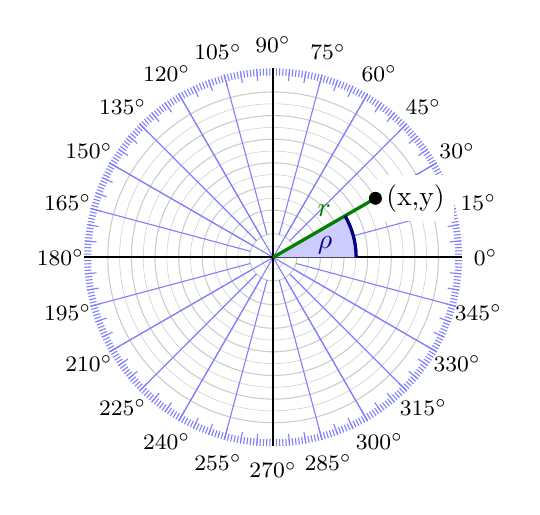
\begin{tikzpicture}[scale=0.3]
    % Circles
    \foreach \r in {1, 2,...,7}
    \draw[black!20] (0,0) circle (\r);
    \foreach \r in {0.5, 1.5,...,7}
    \draw[black!20, very thin] (0,0) circle (\r);
    % 1° Rays
    \foreach \a in {0, 1,...,359}
    \draw[blue!50!white, thin] (\a:7.7) -- (\a:8);
    % 5° Rays
    \foreach \a in {0, 5,...,359}
    \draw[blue!50!white, thin] (\a:7.5) -- (\a:8);
    % 15° Rays
    \foreach \a in {0, 15,...,359}
    \draw[blue!50!white] (\a:1) -- (\a:8);
    % 30° Rays
    \foreach \a in {0, 30,...,359}
    \draw[blue!50!white] (0, 0) -- (\a:8);
    %   % Radius labels (background filled white)
    % \foreach \r in {1, 2,...,7}
    % \draw (\r,0) node[inner sep=1pt,below=3pt,rectangle,fill=white] {$\r$};
    % Main rays
    \foreach \a in {0, 90,...,359}
    \draw[thick] (0, 0) -- (\a:8);
    % Angle labels
    \foreach \a in {0, 15,...,359}
    \draw (\a: 9) node {{\footnotesize $\a^\circ$}};
    % Central point
    \draw[fill=red] (0,0) circle(0.7mm);

    % \filldraw[fill=green!20,draw=green!50!black] (0,0) -- (1,0)
    % arc [start angle=0, end angle=30, radius=1] -- cycle;

    \coordinate (A) at (5,0);
    \coordinate (B) at (0,0);
    \coordinate (C) at (30:5);
    \draw[very thick,green!50!black] (B) -- node[above]{$r$} (C) node[black,right,
    fill=white]{(x,y)}
    pic [draw=blue!50!black, fill=blue!20, angle radius=30] {angle = A--B--C};
    \draw[blue!50!black] (2.2,0.5) node{$\rho$};
   \draw[fill=black] (C) circle(2.5mm);

  \end{tikzpicture}
\end{center}

\end{column}
  \end{columns}

\end{frame}

\begin{frame}
  \frametitle{Spherical Projections}
  \begin{columns}%
    \begin{column}{0.6\textwidth}%
      % In order to visualize spherical data we need to project them onto the
      % plane.

      % \medskip

      % \structure{polar coordinates in the plane:}
      % \begin{equation*}
      %    (x,y) = (r \cos \rho, r
      % \sin \rho)
      % \end{equation*}
      % \structure{polar coordinates on the sphere:}
      % \begin{equation*}
      %   (x,y,z) = (\cos \rho \sin \theta, \sin \rho \sin \theta, \cos \theta)
      % \end{equation*}

      % \medskip
      \vspace{-0.7cm}
        \begin{table}
  \centering
  \begin{tabular}{>{\centering\bfseries}m{1in} >{\centering}m{1in} >{\centering\arraybackslash}m{2in}}
    \toprule
    name & \textbf{formula} & \textbf{schema} \\
    \midrule
    \ul<1|handout:0>{orthographic} & $r=\sin \theta$ &
\includegraphics[height=1.3cm]{pic/ortho}\\ equal angle\\
    \ul<2|handout:0>{\textnormal{(stereographic)}} & $r = \tan \frac{\theta}{2}$
                 & 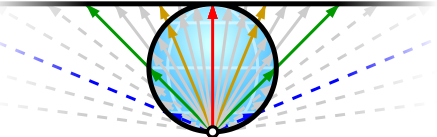
\includegraphics[height=1.3cm]{pic/stereo} \\
    \ul<3|handout:0>{gnonomic} & $r = \tan \theta$ &  
\includegraphics[height=1.3cm]{pic/gnonomic.png}\\[4ex]
    equal area\\
    \ul<4|handout:0>{\textnormal{(Schmidt)}}  & $\sqrt{2(1-\cos\theta)}$ & \\[4ex]
    \ul<5|handout:0>{equal distant}  & $r = \theta$ &\\[1ex]
    \bottomrule
  \end{tabular}
\end{table}

      % \structure{orthographic:} $r=\sin \theta$
      % \structure{stereographic (equal angle):} $r = \tan \frac{\theta}{2}$
      % \structure{gnonomic:} $r = \tan \theta$
      % \structure{Schmidt (equal area):} $r=\sqrt{2(1-\cos\theta)}$
      % \structure{equal distant):} $r = \theta$
      \end{column}%
    \begin{column}{0.4\textwidth}

      % \begin{overlayarea}{\textwidth}{2cm}
      %   \centering
      %   \only<1>{
\includegraphics[height=2cm]{pic/ortho.png}}%
      %   \only<2>{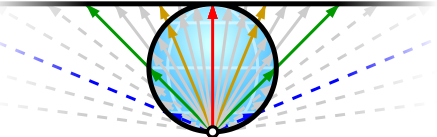
\includegraphics[height=2cm]{pic/stereo}}%
      %   \only<3>{
\includegraphics[height=2cm]{pic/gnonomic.png}}%
      % \end{overlayarea}

      \vspace{3cm}

      \begin{overlayarea}{\textwidth}{5cm}
        \centering
          \only<1|handout:0>{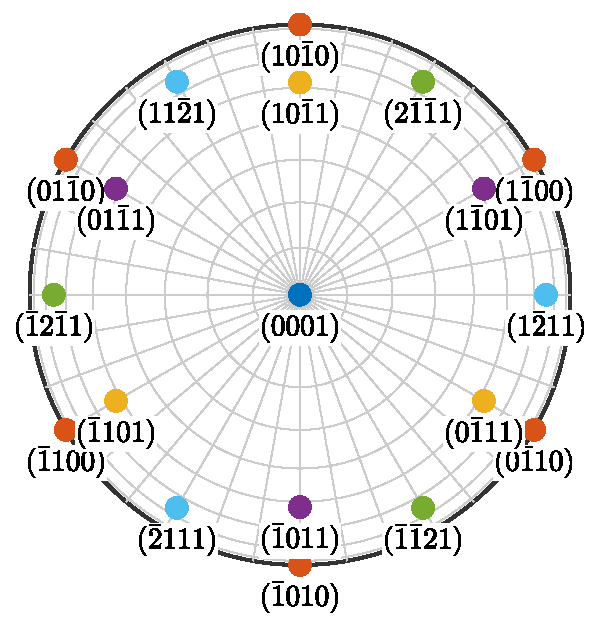
\includegraphics[width=0.8\textwidth]{pic/orthographic}}%
          \only<2>{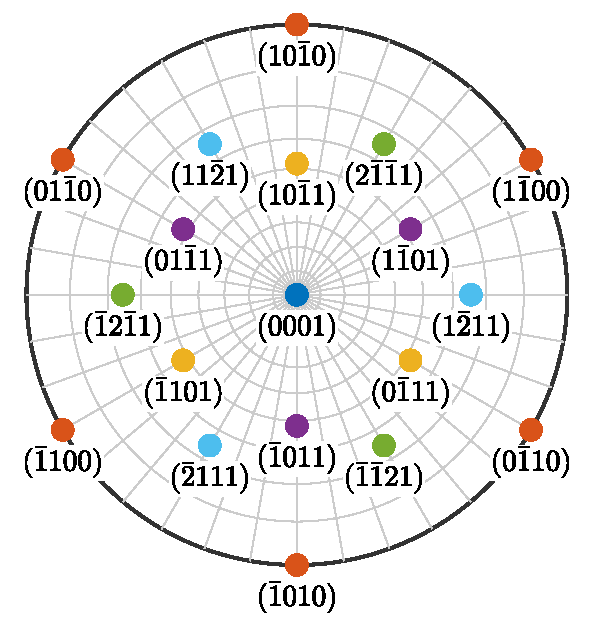
\includegraphics[width=0.8\textwidth]{pic/eangle}}%
          \only<3|handout:0>{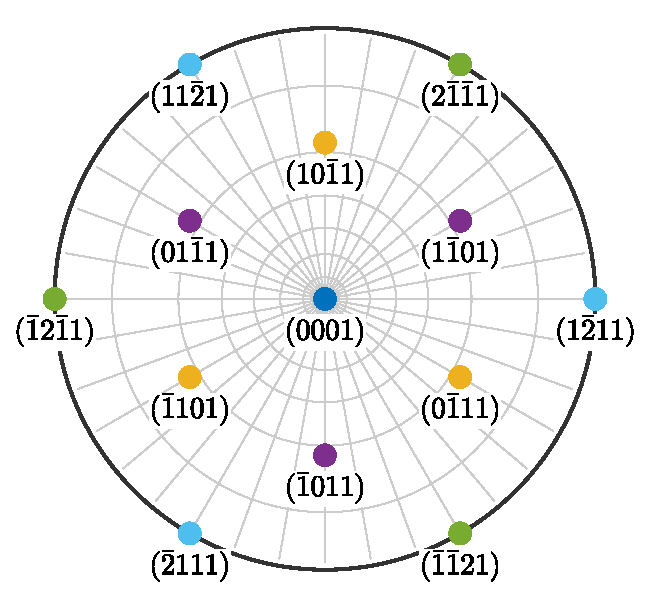
\includegraphics[width=0.8\textwidth]{pic/gnonomic}}%
          \only<4|handout:0>{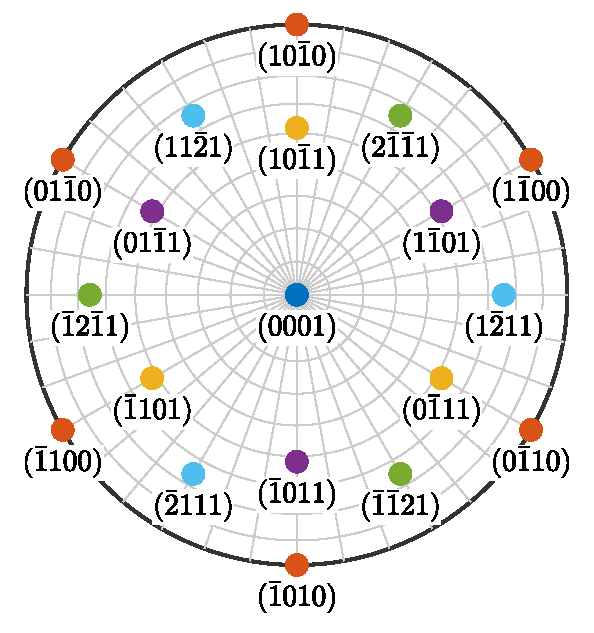
\includegraphics[width=0.8\textwidth]{pic/earea}}%
          \only<5|handout:0>{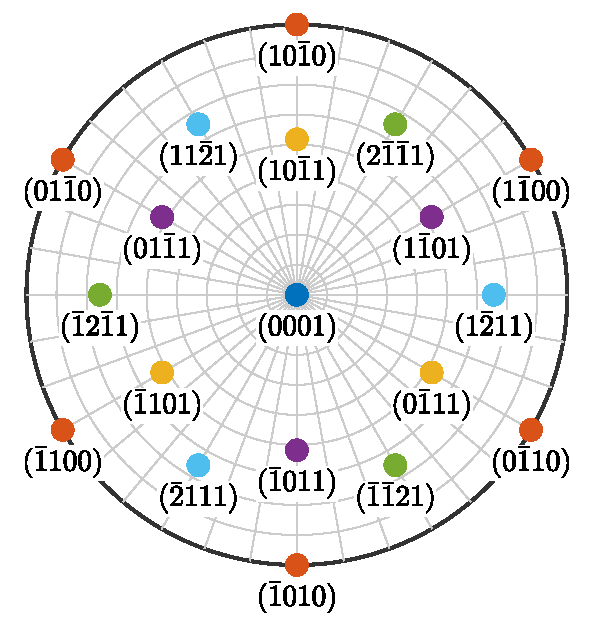
\includegraphics[width=0.8\textwidth]{pic/edist}}
        \end{overlayarea}

    \end{column}
  \end{columns}
\end{frame}


\begin{frame}[fragile]
  \frametitle{Spherical Plots in MTEX}

  \structure{spherical projections:} \texttt{earea, edist, eangle, 3d}

  \bigskip
  \pause

  \structure{spherical region:} \texttt{upper, lower, complete,
    fundamentalRegion}

  \bigskip
  \pause

  \structure{plot alignment:} \texttt{plotx2east, plotx2north, plotzIntoPlane,
    plotzOutOfPlane}

  \bigskip
  \pause

  \structure{\texttt{marker}}: \texttt{s, d, o, v}\\
  \texttt{markerSize, markerEdgeColor, markerFaceColor, linewidth,
    MarkerEdgeAlpha, MarkerFaceAlpha}

  \bigskip
  \pause

  \structure{combined plots:} \texttt{hold on, hold off, add2all}

  \bigskip
  \pause

  \structure{multiple plots:} \texttt{nextAxis, newMTEXFigure, gcm}

  \bigskip
  \pause

  \structure{labels:} \texttt{label, fontSize, backgroundcolor, }

\end{frame}


% \begin{frame}[fragile]
%   \frametitle{Plotting Vectors}

%   \begin{columns}
%     \begin{column}{0.67\textwidth}
%       \begin{overlayarea}{\textwidth}{8cm}

%         spherical projections: \texttt{earea, edist, eangle}
%           \vspace{-0.15cm}
%       %hemisphere: \texttt{upper, lower}
%       \begin{onlyenv}<1>
%         \begin{lstlisting}[style=input]
% plot(r,'projection','eangle','upper')
% \end{lstlisting}
%       \end{onlyenv}
%       \pause
%       \begin{onlyenv}<2->
%         \begin{lstlisting}[style=input]
% plot(r,'projection','earea','upper')
% \end{lstlisting}
%       \end{onlyenv}

% \pause \medskip

% combined plots
% \vspace{-0.1cm}
% \begin{lstlisting}[style=input]
% plot(vector3d(1,1,1),'upper');
% hold on
% plot(vector3d(1,2,3),'label','B');
% plot(vector3d(-1,2,1),'label','A');
% hold off
% \end{lstlisting}

%       \pause \medskip

%       scatter plots
% \vspace{-0.1cm}
%       \begin{lstlisting}[style=input]
% v = vector3d.rand(1000)
% plot(v)
% \end{lstlisting}
% \pause
% contour plots
% \vspace{-0.1cm}
%       \begin{lstlisting}[style=input]
% plot(v,'contourf')
% \end{lstlisting}

%     \end{overlayarea}
%   \end{column}

%   \begin{column}{0.3\textwidth}

%     \begin{overlayarea}{\textwidth}{8cm}
%       \includegraphics<1-2>[width=3.5cm]{pic/vectoreangle}

%       \includegraphics<2>[width=3.5cm]{pic/vectorearea}

%       \includegraphics<3>[width=3.5cm]{pic/vectorCombined}

%       \includegraphics<4>[width=3.5cm]{pic/vectorScatter}

%       \includegraphics<5>[width=3.5cm]{pic/vectorContour}
%     \end{overlayarea}
%   \end{column}
%   \end{columns}

% \end{frame}


% \subsection*{density estimation}

% \begin{frame}[fragile]
%   \frametitle{Density Estimation}

%   Ingredients:
%   \begin{itemize}
%   \item<1-> density function ${\bf \color{green!60!black}f}$
%   \item<2-> vectors ${\color{red!90!black}v_{1}, \ldots,v_{N}}$
%   \end{itemize}

%   \medskip

%   \uncover<3->{ Goal: Find  ${\bf \color{green!60!black}f}$ given ${\color{red!90!black}v_{1}, \ldots,v_{N}}$}

%   \medskip

%   \begin{overlayarea}{\textwidth}{7cm}
%     \center
%     \begin{onlyenv}<1-7>
%       \begin{tikzpicture}
%         \begin{axis}[xtick=-1, ytick=-1,smooth,width=\textwidth, height=7cm, ymin=0,ymax=7,enlargelimits=false]
%           % the true density
%           \addplot[mark=none,very thick,green!60!black] table[x index=0,y index=1]
%           {matlab/example.txt};
%           % the random sample
%           \only<2,3,4,5,6,7>{\addplot[mark=o, only marks, red!90!black] table[x index=0,y index=1]
%           {matlab/sample_1.txt};}
%           % the histogram
%           \only<4>{\addplot[ybar interval, fill=blue!30!white] table[x index=0,y index=1]
%           {matlab/hist.txt};}
%           % the kernel
%           \only<5>{\addplot[mark=none,blue, thick] table[x index=0,y index=22]
%           {matlab/example.txt};}
%           % the kernel density estimator
%           \only<6>{
%             \foreach \x in {4,5,6,...,22}
%             \addplot[mark=none,blue] table[x index=0,y index=\x]
%             {matlab/example.txt};
%           }
%           \only<7>{\addplot[mark=none,blue,very thick] table[x index=0,y index=2]
%             {matlab/example.txt};}
%         \end{axis}
%       \end{tikzpicture}
%     \end{onlyenv}

% %      \only<8>{
% %       \begin{block}{Kernel Density Estimator}
% %         kernel function ${\color{blue!60!black}\mathbf \psi} $
% %         \begin{equation*}
% %           f^{*}(v) = \frac{1}{N} \sum_{n = 1}^N {\color{blue!60!black}\psi}(\mathrm{dist}(v-v_{n})),
% %         \end{equation*}
% %       \end{block}


% %      }
%   \end{overlayarea}
% \end{frame}

% \subsection*{Spherical Functions}


% \begin{frame}[fragile]
%   \frametitle{Spherical Functions}
% %  \begin{columns}
% %    \begin{column}{\textwidth}
%   \begin{overlayarea}{\textwidth}{8cm}
%     evaluate the density at points \texttt{out}
%         \begin{lstlisting}[style=input]
% sF = calcDensity(v,out,'halfwidth',5*degree)
%         \end{lstlisting}

%         \pause

% define a spherical function by density estimation
%         \begin{lstlisting}[style=input]
% sF = calcDensity(v,[],'halfwidth',5*degree)
%         \end{lstlisting}
%       \begin{onlyenv}<2>
%         \vspace{-0.3cm}
%         \begin{lstlisting}[style=output]
% sF = /+spherical function+/ (show methods, plot)

%  vertices: 10088 x 1
%  values:   10088 x 1
% \end{lstlisting}
% \end{onlyenv}

% \begin{onlyenv}<3->
% define a spherical function by interpolation
%   \begin{lstlisting}[style=input]
% sF = interp(v,values)
%   \end{lstlisting}
% \end{onlyenv}


%       \begin{onlyenv}<4>
%         \begin{lstlisting}[style=input]
% plot(sF)
% plot3d(sF)
% [value,v] = max(sF)
% value = sF.eval(v)
% entropy(sF)
% sF = (sF1 + 5*sF2) ./ sF3
%         \end{lstlisting}
%       \end{onlyenv}
%       \end{overlayarea}
% %    \end{column}

% %    \begin{column}{3.5cm}

%   %     \begin{overlayarea}{\textwidth}{8cm}

%   %     \end{overlayarea}
%   %   \end{column}
%   % \end{columns}
% \end{frame}


\begin{frame}[fragile]
  \frametitle{Data Plots}

  \begin{columns}
    \begin{column}{0.67\textwidth}
      colorize vectors by value
        \vspace{-0.15cm}
      \begin{lstlisting}[style=input]
v = vector3d.rand(100)
scatter(v,v.rho./degree)
mtexColorbar southoutside
mtexColorMap hsv
      \end{lstlisting}

      \pause
      \bigskip

      colorize by RGB triples
        \vspace{-0.15cm}
      \begin{lstlisting}[style=input]
key = HSVDirectionKey
scatter(v,key.direction2color(v))
      \end{lstlisting}

      \pause
      \bigskip

      visualize directions
        \vspace{-0.15cm}
      \begin{lstlisting}[style=input]
quiver(v,orth(v)) % a vector field
      \end{lstlisting}
    \end{column}
    \begin{column}{0.3\textwidth}
      \begin{overlayarea}{\textwidth}{8cm}
        \includegraphics<1-2>[width=0.8\textwidth]{pic/vectorColor}
        \includegraphics<2>[width=0.8\textwidth]{pic/vectorRGBColor}
        \includegraphics<3|handout:0>[width=\textwidth]{pic/quiver}
    \end{overlayarea}
    \end{column}
  \end{columns}

\end{frame}

% \subsection*{Annotations}

% \begin{frame}[fragile]
%   \frametitle{Customize Plots}

% \begin{columns}
%   \begin{column}{8.5cm}

% \begin{overprint}
%   \onslide<1|handout:0>%
%   General Syntax%
% \begin{lstlisting}[style=input]
% plot(vector3d,<options>)
% \end{lstlisting}
%   \onslide<2|handout:1>%
%   General Syntax
% \begin{lstlisting}[style=input]
% annotate(orientation,<options>)
% \end{lstlisting}
% \end{overprint}

% Options
% \begin{lstlisting}[style=input]
% Marker            % marker shape
% MarkerSize        % marker size
% MarkerFaceColor   % face color
% MarkerEdgeColor   % edge color
% label             % a label text
% color, background % text colors
% \end{lstlisting}

% \begin{overprint}
%   \onslide<1|handout:0>%
%   Example
% \begin{lstlisting}[style=input]
% plot([vector3d.X,vector3d.Y,vector3d.Z],
%  'Backgroundcolor','w','Marker','s',
%  'MarkerEdgeColor','w','labeled',
%  'MarkerFaceColor','k')
% \end{lstlisting}

%   \onslide<2|handout:1>
% Example
% \begin{lstlisting}[style=input]
% plot(q0,'label','A',...
%  'Backgroundcolor','w','Marker','s',
%  'MarkerEdgeColor','w',...
%  'MarkerFaceColor','r')
% \end{lstlisting}

% \end{overprint}

% \end{column}

% \begin{column}{3.5cm}
%     \onslide<1->
%     \only<1|handout:0>{%
%     \includegraphics[width=3.5cm]{pic/annotationv}%
%     }%
%     \only<2>{%
%     \includegraphics[width=3.3cm]{pic/annotationq}%
%     }%
% \end{column}

% \end{columns}

% \end{frame}

\begin{frame}[fragile]
  \frametitle{Axes}

  \begin{columns}
    \begin{column}{0.67\textwidth}
      \begin{overlayarea}{\textwidth}{8cm}
        Axes are three dimensional vectors where we do not care about length and
        direction, e.g. plane normals.
\begin{lstlisting}[style=input]
r = vector3d(1,1,1,'antipodal')
\end{lstlisting}
\begin{onlyenv}<1|handout:0>
  \vspace{-0.3cm}
\begin{lstlisting}[style=output]
r = /+vector3d+/ (show methods, plot)
 size: 1 x 1
 antipodal: true
  x y z
  1 1 1
\end{lstlisting}
\end{onlyenv}

\medskip
\pause

Then \textbf{\texttt{r}} and \textbf{\texttt{-r}} represent the same axis
\begin{lstlisting}[style=input]
eq(r, -r)
\end{lstlisting}
\begin{onlyenv}<2|handout:0>
  \vspace{-0.3cm}
\begin{lstlisting}[style=output]
  1
\end{lstlisting}
\end{onlyenv}

\medskip
\pause

The angle to an axis is always less then $90^{\degree}$
\begin{lstlisting}[style=input]
angle(r,-vector3d.X) / degree
\end{lstlisting}
\begin{onlyenv}<3|handout:0>
  \vspace{-0.3cm}
\begin{lstlisting}[style=output]
  54.7
\end{lstlisting}
\end{onlyenv}

\medskip
\pause

Changing option \textbf{antipodal}
\begin{onlyenv}<4|handout:0>
\begin{lstlisting}[style=input]
r = vector3d.rand(100)
o = v.orth;
quiver(v,o)
\end{lstlisting}
\end{onlyenv}
\begin{onlyenv}<5>
\begin{lstlisting}[style=input]
r = vector3d.rand(100)
o = v.orth;
o.antipodal = true;
quiver(v,o)
\end{lstlisting}
\end{onlyenv}
\end{overlayarea}
\end{column}
  \begin{column}{0.3\textwidth}
    \only<1-3>{
      \centering
      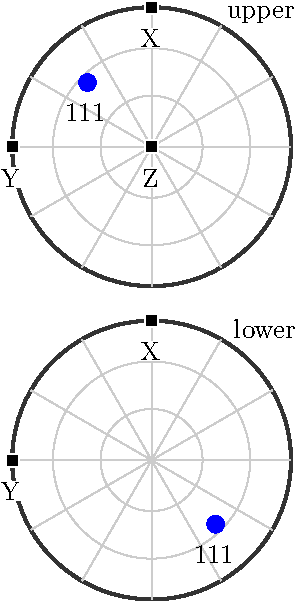
\includegraphics[width=3.5cm]{pic/vectorAntipodal}
    }

    \begin{onlyenv}<4-5|handout:0>
      \begin{overlayarea}{\textwidth}{0.8\textheight}
        \centering{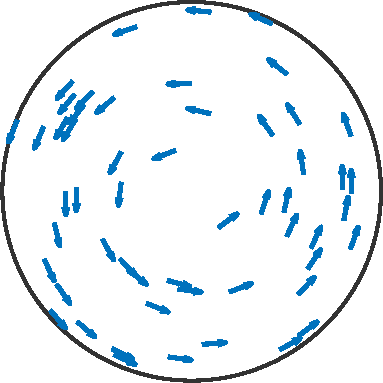
\includegraphics[width=3.5cm]{pic/vecQuiver}}

        \bigskip

        \only<5>{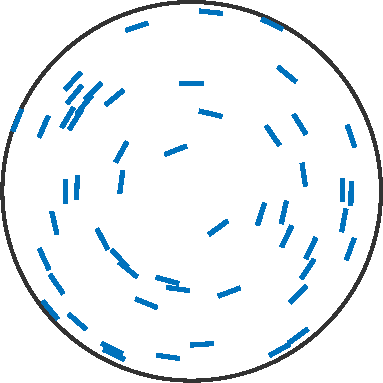
\includegraphics[width=3.5cm]{pic/axesQuiver}}
      \end{overlayarea}
    \end{onlyenv}

  \end{column}
\end{columns}


\end{frame}

\end{document}
